\documentclass{article}
\usepackage[submission]{colm2026_conference}

\usepackage{microtype}
\usepackage{graphicx}
\usepackage{booktabs}
\usepackage{float}
\usepackage{amsmath,amssymb}
\usepackage[colorlinks=true, allcolors=blue]{hyperref}
\usepackage{url}

\input{math_commands.tex}
% AUTO-GENERATED by figure-gen.py from md5-asserted raws. Do not edit.
\newcommand{\tableone}{
\begin{tabular}{lccccc}
\toprule
arm & seed 0 & seed 1 & seed 2 & mean & clears bar? \\
\midrule
matrix fast-weight & 0.9995 & 1.0000 & 0.9990 & 0.9995 & every seed \\
flat-vector recurrence & 0.0322 & 0.0327 & 0.0369 & 0.0339 & never \\
transformer (uncapped) & 0.0271 & 0.0293 & 0.0286 & 0.0283 & never \\
\midrule
\multicolumn{6}{l}{$\Delta$ vs flat-vector: mean 0.9656, 95\% paired CI (0.9582, 0.9729); excludes 0.30} \\
\multicolumn{6}{l}{$\Delta$ vs transformer: mean 0.9712, 95\% paired CI (0.9685, 0.9738); excludes 0.30} \\
\bottomrule
\end{tabular}}
\newcommand{\tablecapped}{
\begin{tabular}{lccc}
\toprule
arm / KV budget & $T{=}454$ & $T{=}902$ & $T{=}1798$ \\
\midrule
contender, fixed 32{,}768 B & 0.9989 & 0.9989 & 0.9989 \\
transformer, uncapped & 0.0293 & 0.0314 & 0.0339 \\
transformer, $M{=}32$ cap & 0.0300 & 0.0251 & 0.0256 \\
transformer, $M{=}16$ cap & 0.0280 & 0.0240 & 0.0251 \\
transformer, $M{=}8$ cap & 0.0257 & 0.0264 & 0.0250 \\
transformer, $M{=}4$ cap & 0.0251 & 0.0277 & 0.0251 \\
transformer, $M{=}2$ cap & 0.0251 & 0.0286 & 0.0257 \\
\midrule
\multicolumn{4}{l}{per-$M$ paired-gap CI lower bounds at $T{=}902$: all $\geq 0.9586$} \\
\bottomrule
\end{tabular}}
\newcommand{\tabletaps}{
\begin{tabular}{llcccc}
\toprule
arm & linear read-out site & cos.\ mean & rf@0.9 & shuffled cos.\ & gap \\
\midrule
contender & $S_1 q$ (shallow query) & 0.165 & 0.000 & 0.105 & +0.060 \\
contender & $S_0 q$ (bind-path query) & 0.118 & 0.000 & 0.112 & +0.006 \\
contender & $S_1 q$ (true query) & 0.167 & 0.000 & 0.104 & +0.063 \\
contender & pre-LM-head hidden & 0.894 & 0.674 & 0.094 & +0.800 \\
\midrule
flat-vector & $S_1 q$ (shallow query) & 0.117 & 0.000 & 0.112 & +0.005 \\
flat-vector & $S_0 q$ (bind-path query) & 0.113 & 0.000 & 0.111 & +0.002 \\
flat-vector & $S_1 q$ (true query) & 0.118 & 0.000 & 0.113 & +0.005 \\
flat-vector & pre-LM-head hidden & 0.119 & 0.000 & 0.112 & +0.006 \\
\bottomrule
\end{tabular}}
\newcommand{\tabletasktwo}{
\begin{tabular}{lccccccccc}
\toprule
arm & s0 & s1 & s2 & s3 & s4 & s5 & s6 & s7 & s8 \\
\midrule
contender & 0.040 & 0.029 & \textbf{0.334} & 0.036 & 0.031 & \textbf{0.479} & 0.028 & \textbf{0.391} & 0.041 \\
flat-vector & 0.034 & 0.028 & 0.037 & 0.031 & 0.031 & 0.032 & 0.034 & 0.031 & 0.035 \\
\midrule
\multicolumn{10}{l}{pooled paired $\Delta$ CI (-0.020, 0.268), flagged non-decision-grade (var-ratio 6.14$>$4.0)} \\
\bottomrule
\end{tabular}}
\newcommand{\tablekstress}{
\begin{tabular}{lccc}
\toprule
 & matrix fast-weight & flat-vector & transformer \\
\midrule
$K{=}48$ ($K/d{=}0.75$) accuracy & 0.0189 & 0.0195 & 0.0218 \\
\multicolumn{4}{l}{chance 0.0208; locate-only bar 0.0625; no arm clears} \\
\bottomrule
\end{tabular}}
\newcommand{\nparamscontender}{14{,}049{,}408}
\newcommand{\nparamsablation}{14{,}048{,}384}
\newcommand{\nparamstransformer}{14{,}440{,}448}


\title{Constant-Memory Recall: A Fixed 32\,kB Fast-Weight State Retains
In-Context Bindings That a Matched Transformer Does Not Learn}

\author{Anonymous authors}

\begin{document}

\maketitle
% Running head: the official COLM kit's submission mode prints "Under
% review as a conference paper at COLM 2026"; this submission targets the
% Efficient Reasoning workshop, which mandates the COLM format but is not
% the main conference. Header text only; no format rule (margins, fonts,
% title block) is altered.
\lhead{Under review at the Workshop on Efficient Reasoning, COLM 2026}

\begin{abstract}
Long-horizon inference is increasingly memory-bound: a transformer's
key--value (KV) cache grows linearly with
context length, while fast-weight recurrences carry a state of fixed size.
Whether such a state retains the bindings a recall task depends on, under a
training budget an attention model also receives, is an empirical question.
We compare three models matched in parameters, data, and training schedule
on episode-restricted 32-way associative recall: a two-block matrix
fast-weight model holding 32{,}768 bytes of recurrent
state, % <!-- evidence: C10 -->
a flat-vector recurrence, and a transformer. The fast-weight model answers recall queries
at 0.9995 mean accuracy over three seeds; % <!-- evidence: C1 -->
both baselines sit at chance, and paired-seed confidence intervals exclude
the pre-registered 0.30 separation margin with lower bounds above
0.95. % <!-- evidence: C2 -->
Accuracy stays at or above 0.998 for every seed when the same episode is
embedded in contexts of 454 to 1{,}798 tokens, eight times the binding
span, with the state fixed at 32{,}768 bytes; % <!-- evidence: C3 -->
the transformer reads chance uncapped and at every KV-cache budget from one
to thirty-two times those bytes, % <!-- evidence: C4 -->
so no memory multiplier is claimed and the baseline is reported as
non-competitive at the matched budget. State-zeroing localizes the recall
to the first block's fast-weight state. % <!-- evidence: C5 -->
A multi-hop variant separates only as seed variance, and at higher load
every arm reads chance. % <!-- evidence: C7 -->
\end{abstract}

\section{Introduction}

Serving a transformer over a long context is a memory problem before it is a
compute problem. The KV cache of a decoder-only model
\citep{vaswani2017attention} grows linearly with context length, and at
deployment scale that growth, not arithmetic throughput, sets the limit on
batch size, context window, and cost. A substantial literature therefore
compresses or evicts cache entries \citep{xiao2023efficient, zhang2023h2o},
trading recall fidelity for bytes held.

Fast-weight recurrences occupy the opposite corner of this trade. A model
whose mixer maintains a matrix state updated by an outer-product rule
\citep{schmidhuber1992learning, ba2016using, schlag2021linear,
katharopoulos2020transformers, yang2024parallelizing, gu2023mamba} carries a
memory of fixed byte size regardless of context length. The architecture
promises constant-memory inference, but the promise rests on an empirical
premise that is rarely tested head to head: that the fixed state, trained
under the same budget an attention model receives, in fact retains the
bindings a long-horizon task queries. Prior diagnostic work has, if
anything, pointed the other way; on multi-query associative recall,
attention models dominate efficient recurrent alternatives when both are
trained well \citep{arora2023zoology}.

We report a matched-budget comparison in which the fixed state wins, and
wins at ceiling. On episode-restricted 32-way associative recall, a
two-block matrix fast-weight model whose entire recurrent state occupies
32{,}768 bytes % <!-- evidence: C10 -->
answers queries at 0.9995 mean accuracy over three seeds, % <!-- evidence: C1 -->
while a parameter-matched flat-vector recurrence and a parameter-matched
transformer, trained on identical data for identical steps, both sit at
chance. % <!-- evidence: C1 -->
The paired-seed confidence intervals exclude the pre-registered 0.30
separation margin with lower bounds above 0.95. % <!-- evidence: C2 -->
The separation survives context extension: with the state fixed at
32{,}768 bytes, accuracy stays at or above 0.998 for every seed as the same
episode is embedded at 454, 902, and 1{,}798 tokens, % <!-- evidence: C3 -->
and the transformer stays at chance both uncapped and under every KV-cache
byte budget from $1\times$ to $32\times$ the fast-weight state. % <!-- evidence: C4 -->

Because the baseline never demonstrates recall at any cache budget, the
comparison licenses no ``$M\times$ less memory'' headline. We follow the
pre-registered analysis rule for this case and report the registered
outcome verbatim: \emph{baseline non-competitive at matched
params/tokens}. % <!-- evidence: C4 -->

Our contributions:
\begin{itemize}
\item \textbf{A matched three-arm separation on recall.} Parameters matched
  within 2.8\%, % <!-- evidence: C9 -->
  identical tokens, steps, optimizer, and paired episode seeds; the
  fast-weight arm clears the demonstration bar in every seed, the baselines
  never do (Section~\ref{sec:recall}).
\item \textbf{A constant-memory demonstration.} Recall accuracy is flat in
  context length out to eight times the binding
  span % <!-- evidence: C3 -->
  at a fixed 32{,}768-byte
  state, % <!-- evidence: C10 -->
  while no KV budget up to $32\times$ those bytes
  rescues the transformer % <!-- evidence: C4 -->
  (Section~\ref{sec:horizon}).
\item \textbf{A causal mechanism read.} Zeroing the first block's
  fast-weight state collapses recall to chance in every seed, the second
  block's state proves inert, and no linear probe on either raw state
  decodes the bindings, so the storage is nonlinear and the model's own
  forward pass is its decoder (Section~\ref{sec:mechanism}).
\item \textbf{Scope, disclosed.} A multi-hop variant of the task is a
  trainability finding, not a capability separation (3 of 9 contender
  seeds learn it; 0 of 9 baseline seeds), % <!-- evidence: C7 -->
  and at load $K/d = 0.75$ every arm reads chance % <!-- evidence: C8 -->
  (Section~\ref{sec:scope}).
\end{itemize}

\section{Experimental setup}
\label{sec:setup}

\subsection{Task: episode-restricted associative recall}

Each training and evaluation sequence is an \emph{episode}: $K = 32$ bind
clauses followed by a query. A bind clause is a 7-token statement linking a
key entity to a value entity, both drawn without replacement from a pool of
real GPT-2 token identifiers \citep{radford2019language}, so the binding
span is $T_{\mathrm{bind}} = K \times 7 = 224$
tokens. % <!-- evidence: C10 -->
The query names one key; the model must produce the bound value at the
answer position. Keys and values are re-drawn every episode, so the map is
in-context and cannot be memorized in slow weights. The primary task is
single-hop; a multi-hop variant appears in Section~\ref{sec:scope}.

\textbf{Metric.} We score \emph{episode-restricted recall accuracy}: the
argmax over the model's own LM-head logits restricted to the episode's $K$
bound values, read at the answer position of the model's own continuation.
Chance is $1/K = 0.03125$, and an arm counts as demonstrating recall in a
cell only above the pre-registered demonstration bar of $3/K = 0.09375$;
readings at or below the bar are scored no-recall, and differences between
two no-recall arms are treated as chance-level noise ordering, never as
separation. One caveat travels with every accuracy in this paper: under
argmax decoding, an associative state of rank one can already support on
the order of $d$ associations \citep{nichani2024understanding}, so recall
accuracy here never establishes rank, continuous recovery, or storage
capacity. Section~\ref{sec:mechanism} reports the continuous-readout
diagnostics separately.

\subsection{Three arms, matched budget}

\textbf{Matrix fast-weight model (the contender).} A two-block
decoder-style LM whose mixer holds
a $64 \times 64$ matrix state $S_t$ per block, updated by a delta rule
\citep{schlag2021linear, yang2024parallelizing}:
$S_t = S_{t-1}(I - \beta_t k_t k_t^{\top}) + \beta_t v_t k_t^{\top}$, with
per-token read $o_t = S_t q_t$. Its total recurrent state is
$2 \times 64 \times 64$ fp32 values, or 32{,}768 bytes, constant in context
length. % <!-- evidence: C10 -->

\textbf{Flat-vector recurrence (the additive control).} Identical
embedding table, output head, and feed-forward blocks; only the mixer
changes, to a gated elementwise vector recurrence
$s_t = s_{t-1} \odot g_t + v_t$ with read $o_t = s_t \odot q_t$, at matched
total parameter count via mixer width and $d_{\mathrm{state}} = 64$ pinned
equal to the contender's. This arm removes the multiplicative
outer-product update while preserving everything else, rather than
reshaping the same operator, since any $d^2$-dimensional vector can encode
a $d \times d$ matrix and structure matters only if the operations use it.
This control differs from the contender on three axes at once: mixer
recurrence, raw state capacity (512 bytes versus 32{,}768,
% <!-- evidence: C10 -->
reported for completeness), and write conditioning. Its update has no
dependence on the key $k_t$ at all, so it cannot perform
content-addressed binding under any training outcome. Vector-native
schemes that do bind from a vector state use a key-dependent operation,
circular convolution \citep{plate1995holographic} or tensor-product
binding \citep{smolensky1990tensor}; this control has none.
Section~\ref{sec:recall} states which reading of the resulting
comparison the capacity and write-conditioning gaps permit.

\textbf{Transformer.} A two-layer GPT-2-style causal decoder with the same
tokenizer and width, evaluated in two roles: uncapped (its full KV cache),
and KV-capped with attention-sink-plus-FIFO eviction
\citep{xiao2023efficient} at a total cache budget pinned to
$M \times 32{,}768$ bytes across all layers and heads, swept over
$M \in \{1, 2, 4, 8, 16, 32\}$. % <!-- evidence: C10 -->

Parameter counts are \nparamscontender{} (contender), \nparamsablation{}
(flat-vector, $-0.007\%$), and \nparamstransformer{} (transformer,
$+2.8\%$). % <!-- evidence: C9 -->
All arms train from scratch for 20{,}000 steps at learning rate
$3 \times 10^{-4}$ with the same optimizer, batch schedule, auxiliary
losses, and episode stream; sampling seeds are paired across arms, so the
three arms of a given seed index see identical
episodes. % <!-- evidence: C9 -->

\subsection{Analysis protocol, frozen before the runs}

Margins, tiers, and analysis rules were registered in the project's
experiment registry and frozen before the multi-seed runs. The primary
comparison is contender versus flat-vector at the matched final
checkpoint: a win requires the contender to clear the demonstration bar
and the paired-seed 95\% $t$-interval on the accuracy difference (three
seeds, $\mathrm{df}=2$) to exclude a 0.30 margin. Two clauses matter for
reading this paper. First, the registry pins a \emph{degenerate-baseline}
rule: if the uncapped transformer itself fails the demonstration bar at
the primary cell, the capped-budget walk is definitionally degenerate,
every cap is trivially cleared, and the registered outcome is ``baseline
non-competitive at matched params/tokens,'' with no memory-multiplier tier
certified. Second, a joint-no-recall rule scores any cell where both
compared arms sit at the bar as a tie, never as a separation. Evaluation
uses a pinned held-out query set of 4{,}096 queries over 128 episodes per
cell, % <!-- evidence: C3 -->
identical across arms and seeds. Three seeds is the registered count for
the primary comparison; the protocol includes a seed-extension trigger
for any cell whose paired gap approaches the 0.30 margin, and none did
(Table~\ref{tab:main}), % <!-- evidence: C2 -->
so the count was not extended for this comparison. The multi-hop
variant's later nine-seed table (Section~\ref{sec:scope}) reflects a
different, seed-variance-driven extension under the same protocol, not a
change in standard. The protocol treats the primary
contender-versus-additive-control comparison as the single
pre-registered decision rule; the remaining reported intervals in this
paper (the per-$M$ capped-budget gaps, the pooled multi-hop interval,
per-seed bar comparisons) are descriptive and diagnostic rather than
additional hypothesis tests, so no multiple-comparison correction is
applied to them.

\section{Recall separation at matched budget}
\label{sec:recall}

\begin{table}[t]
\centering
\small
\tableone
\caption{Episode-restricted recall accuracy on the primary cell ($K=32$,
$K/d=0.5$, binding span 224 tokens), per seed and mean, at the matched
final checkpoint (20{,}000 steps, identical data and optimizer; chance
$1/32 = 0.031$, demonstration bar $3/32 = 0.094$). The matrix fast-weight
model clears the bar in every seed; neither the parameter-matched
flat-vector recurrence nor the parameter-matched uncapped transformer ever
does. Both paired-seed 95\% $t$-intervals ($\mathrm{df}=2$) exclude the
pre-registered 0.30 margin. Accuracy is argmax-decoded and
episode-restricted, so it carries the capacity caveat of
Section~\ref{sec:setup}.}
\label{tab:main}
\end{table}

Table~\ref{tab:main} reports the primary comparison. The contender reads
0.9995, 1.0000, and 0.9990 across the three seeds, % <!-- evidence: C1 -->
at least $10\times$ the demonstration bar in every seed; the flat-vector
arm reads 0.0322 to 0.0369 and the transformer 0.0271 to 0.0293, all
within noise of chance and below the bar in every
seed. % <!-- evidence: C1 -->
The paired difference against the flat-vector arm is 0.9656 with a 95\%
interval of $(0.9582,\, 0.9729)$; against the transformer, 0.9712 with
$(0.9685,\, 0.9738)$. % <!-- evidence: C2 -->
Both intervals exclude the frozen 0.30 margin with more than 0.65 to spare
at the interval floor, and no seed straddle fires the registered
seed-extension trigger. % <!-- evidence: C2 -->

The readings this table supports are narrower than the raw gap suggests.
Under the shared training budget, the matrix fast-weight update reaches
ceiling while the additive control's training loss barely moves past its
first-500-step value for the remaining 97.5\% of the run
(Appendix~\ref{app:traincurve}); learning rate, warmup, and
auxiliary-loss weighting were shared across three architecturally
distinct mixers, not independently tuned per arm, so this paper does not
claim the additive update is \emph{architecturally incapable} of the
task, only that it does not reach it under this budget. A second reading
holds but is more modest than ``matrix beats vector'': the additive
control also holds $64\times$ less raw state and a write with no
dependence on the query key (Section~\ref{sec:setup}), so the comparison
shows \emph{a matrix state with a multiplicative, key-conditioned
write outperforms a smaller, non-key-conditioned vector state under a
shared training budget}; capacity and write-conditioning are not
disentangled by this ablation, and no resized or key-conditioned vector
control was run. The transformer column carries its registered phrasing,
\emph{non-competitive at matched params/tokens}: at this scale and budget
it does not learn the task at all, which is itself the axis-2 datum,
never extrapolated to differently-scaled or differently-trained attention
models. What the table does not license is any claim that a transformer
\emph{cannot} perform this task, or that outer-product structure
specifically, rather than capacity and key-conditioning together, is
what the additive control's failure isolates. Attention solves
associative recall well in other regimes \citep{arora2023zoology,
nichani2024understanding}; under this task distribution, tokenizer,
parameter count, and step count, the attention arm did not get there
while the fast-weight arm reached ceiling in every seed.

\section{A fixed state versus a growing cache at long horizon}
\label{sec:horizon}

\begin{figure}[t]
\centering
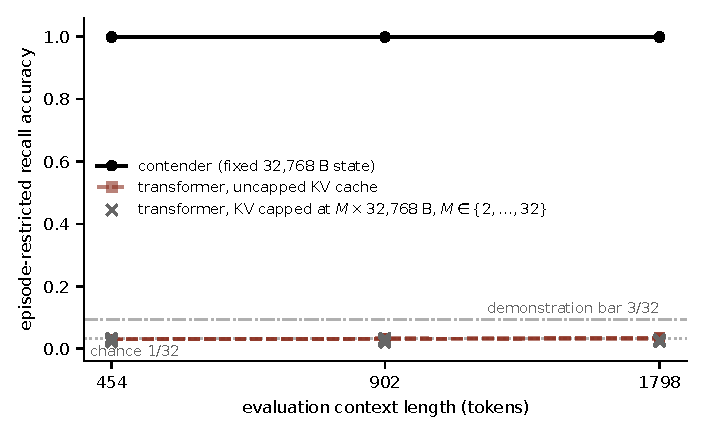
\includegraphics[width=0.86\linewidth]{figures/fig1_horizon.pdf}
\caption{Episode-restricted recall accuracy versus evaluation context
length (log scale) on the primary cell. Each episode's 224-token binding
span is embedded in filler continuation out to 454, 902, and 1{,}798
tokens. The matrix fast-weight model (three seeds, solid) holds
$\geq 0.998$ at every horizon with its state fixed at 32{,}768 bytes. The
transformer reads chance at every horizon, both uncapped (dashed) and
under sink-plus-FIFO KV caps at $M \times 32{,}768$ bytes for
$M \in \{2, \ldots, 32\}$ (crosses; $M{=}1$ is excluded from the walk
because its 8-token cap sits below the query length and is reported
descriptively in Table~\ref{tab:capped}). Reference lines mark chance
($1/32$) and the pre-registered demonstration bar ($3/32$).}
\label{fig:horizon}
\end{figure}

The constant-memory question is whether the recall of
Section~\ref{sec:recall} survives when the bound episode sits inside a
much longer context, with the fast-weight state's byte size unchanged. We
re-evaluate the same frozen checkpoints with each episode embedded in
filler continuation at three horizons: 454, 902, and 1{,}798 tokens, that
is, two, four, and eight times the binding span plus the
query. % <!-- evidence: C3 -->

\textbf{The fixed state does not decay.} The contender reads 0.9995,
0.9983, and 0.9990 (per seed) at \emph{every} horizon; the three curves in
Figure~\ref{fig:horizon} are flat to the third decimal from 454 to 1{,}798
tokens. % <!-- evidence: C3 -->
The state occupies 32{,}768 bytes at every point on the
curve. % <!-- evidence: C10 -->

\textbf{No cache budget rescues the baseline.} The uncapped transformer
reads 0.029 to 0.036 across seeds and horizons; % <!-- evidence: C4 -->
capped at every budget $M \times 32{,}768$ bytes for
$M \in \{2, \ldots, 32\}$ it reads 0.020 to 0.033, at or below its own
uncapped reading everywhere. % <!-- evidence: C4 -->
Per the frozen no-recall rule, these differences are chance-level
orderings. Two registered hypotheses die here at once. A larger cache
does not eventually hold the bindings: $M{=}32$ grants the cache more
bytes than the episode needs and the reading does not move. Forced
locality, which might have \emph{helped} by concentrating attention on
recent tokens, does not either; every capped reading sits at or below
uncapped.

\textbf{What is not claimed.} The registered degenerate-baseline clause
fires on this data exactly as written: the uncapped baseline itself fails
the demonstration bar at the primary cell (readings 0.0271 to 0.0293),
% <!-- evidence: C4 -->
so every cap is trivially cleared and the per-$M$ walk cannot certify a
memory-multiplier tier. Although each of the five eligible per-$M$ paired
gaps is individually clean (interval lower bounds all $\geq 0.9586$ at the
902-token decision horizon), % <!-- evidence: C4 -->
we quote no ``the fast-weight model matches at $M\times$ less memory''
figure, because there is no competent baseline reading to anchor the
ratio. The registered outcome is the sentence used throughout this paper:
baseline non-competitive at matched params/tokens. What the comparison
yields instead is the contender's flat horizon curve at constant bytes,
together with the failure of every cap to change the baseline.
Table~\ref{tab:capped} in the appendix lists the full grid.

\section{Where the recall lives}
\label{sec:mechanism}

\begin{figure}[t]
\centering
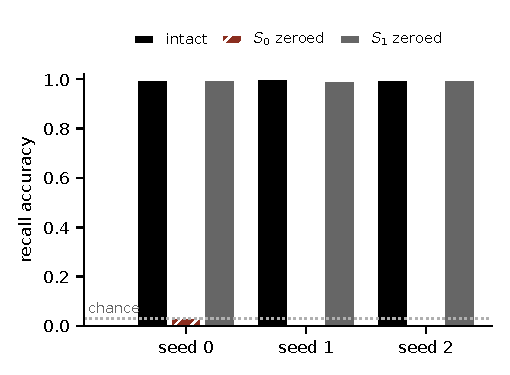
\includegraphics[width=0.62\linewidth]{figures/fig2_szero.pdf}
\caption{Causal state-zeroing on the matrix fast-weight model, per seed on
the primary cell (4{,}096 pinned queries per read; chance $1/32$). Zeroing
the first block's fast-weight state $S_0$ before the query continuation
collapses recall to chance; zeroing the second block's state $S_1$ leaves
it within noise of intact. The bindings are causally resident in $S_0$.}
\label{fig:szero}
\end{figure}

A separation on accuracy alone leaves open where the winning arm keeps the
bindings. We intervene directly: after the bind phase, the recurrent
states are frozen, one block's state is replaced with zeros, and the query
continuation runs as a pure function of the remaining state and the query
tokens. The decoder reads only the state, never the raw bind tokens, and
this is checked rather than assumed: a fresh model instance given only
the cached state (no raw bind-phase tokens) reproduces bit-identical
continuation logits to the original run, closing the channel by which a
hidden cache of the raw tokens could otherwise leak into the query pass.

\textbf{The first block's state is causally necessary; the second block's
is inert.} Zeroing $S_0$ collapses per-seed accuracy from 0.9995, 1.0000,
0.9990 to 0.0339, 0.0012, 0.0002; % <!-- evidence: C5 -->
zeroing $S_1$ leaves 0.9995, 0.9949, 0.9990. % <!-- evidence: C5 -->
The same intervention on the flat-vector arm collapses its already-chance
reading no further, and the pattern replicated in all twelve recurrent
cells of the multi-seed run without a single localization
failure. % <!-- evidence: C5 -->
One instrument note: at seed 1 (intact accuracy exactly 1.0),
$S_1$-zeroing produces a small, reproducible change on 21 of 4{,}096
queries (0.51\%, $\Delta = 0.0051$). % <!-- evidence: C5 -->
The binomial standard-error band used elsewhere in this check assumes a
sampling process and is ill-posed at $p = 1$ (it evaluates to zero
width); both the intact and $S_1$-zeroed readings are deterministic
argmax decodes of the same frozen checkpoint on the same fixed query
set, so there is no sampling process for the band to characterize, the
21-query change is a real and repeatable effect of the intervention,
and the band is not used to adjudicate this cell. The effect does not touch the $S_0$-necessity
result; whether those 21 queries reflect a small, consistent causal
contribution from $S_1$ or near-tied logits is not established by this
instrument. % <!-- evidence: C5 -->

\textbf{The storage is nonlinear, and the model's own forward pass is
its decoder.} Ridge probes fit offline on 24{,}576 fresh draws and evaluated
on the pinned query set recover the bound value's target vector from
\emph{no} linear read-out of either raw state: every $(S, q)$ combine
tested, including one placed directly on the causally necessary $S_0$,
reads within at most a $+0.063$ cosine gap of its shuffled control and
passes a 0.9 cosine threshold on 0.0\% of queries. % <!-- evidence: C6 -->
Only the post-second-block, pre-LM-head hidden state is linearly
decodable, and only in the fast-weight arm: cosine mean 0.894, threshold
pass rate 0.674, gap $+0.800$ over its shuffled
control. % <!-- evidence: C6 -->
The flat-vector arm's same site reads 0.119, pass rate
0.0. % <!-- evidence: C6 -->
The bindings therefore live in $S_0$ in a format no tested linear map
exposes; what transforms the $S_0$-derived signal into a linearly
legible code is the second block's own forward computation, since its
recurrent state is causally inert (Figure~\ref{fig:szero}). Consistent
with a nonlinear store read through a learned decoder, the pass rate of
the pre-LM-head probe varies across seeds (0.686, 0.771, 0.951) while
task accuracy is flat at ceiling; % <!-- evidence: C6b -->
probe legibility is a property of the instrument.
Appendix Table~\ref{tab:taps} lists all read-out sites.

\section{Scope: what does not separate}
\label{sec:scope}

Two further results bound the claim.

\begin{table}[t]
\centering
\small
\tabletasktwo
\caption{Multi-hop variant, nine seeds per compared arm, accuracy at the
matched final checkpoint (chance 0.031, demonstration bar 0.094; readings
above the bar in bold). Three of nine matrix fast-weight seeds learn the
task; zero of nine flat-vector seeds do. The pooled paired interval
straddles zero and is additionally flagged non-decision-grade by a
pre-registered batch-effect gate, so this table is a trainability
disclosure, not a capability claim.}
\label{tab:task2}
\end{table}

\textbf{Multi-hop recall separates only as seed variance.} On the
multi-hop variant (compositional queries over a single Hamiltonian
$K$-cycle, trained at hop depths 1--2, Table~\ref{tab:task2}), the contender clears the
demonstration bar in 3 of 9 seeds (0.334, 0.479, 0.391) and reads chance
in the other six; the flat-vector arm reads chance in all
nine. % <!-- evidence: C7 -->
The registered adjudication rule scores this as
trainability/seed-variance: the hypothesis that multi-hop recall is a hard
capability boundary for this architecture at this scale is rejected (some
seeds reach it), but the pooled paired interval $(-0.020,\, 0.268)$
straddles zero and the pre-registered batch-effect gate flags the pooled
cohort (variance ratio 6.14 against a 4.0 bound), so no capability
separation is claimed in either direction. % <!-- evidence: C7 -->
The bar-clearing seeds also do not generalize: held-out hop depths 3--4
read chance, and the first bar-clearing seed's partial recall collapses to
0.010 when its episode is embedded at any extended
horizon. % <!-- evidence: C7 -->
Multi-hop composition at this scale remains an open training problem.

\begin{table}[t]
\centering
\small
\tablekstress
\caption{Stress cell at $K{=}48$ bindings on the same $d{=}64$ state
($K/d = 0.75$; chance 0.021). Every arm, including the matrix fast-weight
model, reads chance: the recall separation of Table~\ref{tab:main} is
load-bounded and does not extend to this operating point at this scale
and budget.}
\label{tab:k48}
\end{table}

\textbf{The separation is load-bounded.} At $K = 48$ bindings on the same
64-dimensional state ($K/d = 0.75$, Table~\ref{tab:k48}), all three arms read chance: 0.0189
(contender), 0.0195 (flat-vector), 0.0218
(transformer). % <!-- evidence: C8 -->
This cell was registered as locate-only, so it carries no tier
arithmetic; what it establishes is that the ceiling-level recall at
$K/d = 0.5$ does not come for free at higher load under the same training
budget. Where between the two load points the capability degrades, and
whether more training moves the boundary, are open questions this paper
does not answer.

\section{Related work}
\label{sec:related}

\textbf{Fast-weight memory.} Writing transient associations into
multiplicative weights dates to \citet{schmidhuber1992learning}, revived
for attention-era models by \citet{ba2016using}. \citet{schlag2021linear}
identified linear attention \citep{katharopoulos2020transformers} as a
fast-weight programmer and introduced the delta-rule update our contender
uses; \citet{yang2024parallelizing} made that rule trainable at scale.
Selective state-space models \citep{gu2023mamba} pursue the same
constant-state property with a different recurrence, gated delta rules
refine the contender's own update \citep{yang2024gated}, and test-time
memorization modules \citep{behrouz2024titans} share this paper's
motivating contrast between a fixed-size memory and a growing KV cache.
None of these works
reports a parameter- and token-matched comparison against both a
transformer and a structure-removed vector control on episode-restricted
recall, with a causal state intervention and a byte-pinned cache-cap
protocol; that combination is this paper's contribution.

\textbf{Recall as the diagnostic.} \citet{arora2023zoology} established
multi-query associative recall as the axis separating attention from
efficient alternatives, with the opposite headline: in their regime,
attention wins and recurrent models lag. The two findings are consistent;
ours sits at a different operating point: a small matched budget
(14M-class models, 20{,}000 steps from scratch), higher load per state
dimension ($K/d = 0.5$), an episode-restricted argmax metric, and a task
distribution built for exact matched-budget control. We also report where
our separation dies ($K/d = 0.75$, Section~\ref{sec:scope}), which their
framing predicts it must somewhere.

\textbf{KV-cache reduction.} Sink-plus-window eviction
\citep{xiao2023efficient} and heavy-hitter selection \citep{zhang2023h2o}
compress the cache of a model that already performs the task, asking how
few bytes preserve its behavior. We use the sink-plus-FIFO mechanism of
\citet{xiao2023efficient} in the opposite role, as an evaluation
instrument that pins the baseline's cache to a byte budget matched against
a fixed-size state, and our question is prior to theirs: whether the
matched attention model learns the behavior at all.

\textbf{Associative-memory capacity.} \citet{nichani2024understanding}
analyze factual recall in transformers via associative memories and prove
that under argmax decoding a rank-one outer-product store supports on the
order of $d$ associations. We import their result as a standing caveat on
what accuracy metrics can claim (Section~\ref{sec:setup}); our
contribution is empirical and comparative, not a capacity bound.

\section{Limitations}
\label{sec:limitations}

The models are
14M-parameter class, trained 20{,}000 steps from scratch on a synthetic
episode distribution with a GPT-2 tokenizer; nothing here speaks to
pretrained models, natural text, or other scales. The baseline
non-competitiveness holds at the matched budget only: a larger, longer-,
or differently-trained transformer requires its own matched run before any
extension of the claim. The metric is argmax-decoded and
episode-restricted, so by the capacity results of
\citet{nichani2024understanding} it supports no statement about rank,
exact recovery, or how much the 32{,}768-byte state holds; the continuous
diagnostics of Section~\ref{sec:mechanism} are reported only as
bounds. The separation is demonstrated for one fast-weight family (a
delta-rule matrix state) against one vector control and one transformer
configuration; the multi-hop variant does not separate
(Section~\ref{sec:scope}); and the recall ceiling is load-bounded, with
every arm at chance at $K/d = 0.75$. Horizon evaluation extends context
with filler continuation, not with distractor bindings, which is the
easier long-context condition and is disclosed as such. The longest
tested context is 1{,}798 tokens, eight times the binding
span: % <!-- evidence: C3 -->
this paper demonstrates the constant-memory \emph{mechanism} as a
small-scale existence result, not a claim that it holds at the context
lengths (tens of thousands to millions of tokens) where KV-cache cost is
a practical deployment constraint.

\section{Conclusion}

Under a fully matched training budget, a two-block matrix fast-weight
model stores and retrieves in-context bindings that neither matched
baseline learns at all, from a state whose size does not grow with
context. The bindings are causally localized to the first block's
fast-weight matrix and stored in a form only the model's own forward
pass decodes. A baseline that never becomes competent anchors no ratio,
so no memory multiplier is on offer; the registered outcome of
Section~\ref{sec:horizon} is the paper's only comparative claim. For the
workshop's question, whether long-horizon reasoning must pay a memory
cost that grows with context, this is a small-scale existence result on
the recall substrate such reasoning requires: at matched budget, the
constant-memory architecture was the only one that learned to remember.


\bibliography{refs}
\bibliographystyle{colm2026_conference}

\appendix
\section{Full capped-budget grid}
\label{app:capped}

\begin{table}[H]
\centering
\small
\tablecapped
\caption{Mean episode-restricted recall accuracy (three seeds) by arm, KV
budget, and evaluation context length on the primary cell. The matrix
fast-weight model's state is 32{,}768 bytes at every entry of its row; the
transformer's cap at budget $M$ pins its total KV bytes across layers and
heads to $M \times 32{,}768$. $M{=}1$ is excluded from the registered walk
because its cap length (8 tokens) sits below the query length; its
descriptive readings, 0.021 to 0.030 across seeds and horizons, sit at
chance like every other transformer entry. Chance is 0.031; the
demonstration bar is 0.094; no transformer entry approaches
either.} % <!-- evidence: C4 -->
\label{tab:capped}
\end{table}

\section{Linear read-out sites}
\label{app:taps}

\begin{table}[H]
\centering
\small
\tabletaps
\caption{Offline ridge-probe recovery of the bound value's target vector
by read-out site, on the single-seed localization checkpoints (fit on
24{,}576 fresh draws, evaluated on the pinned 4{,}096-query set;
``rf@0.9'' is the fraction of queries whose predicted vector clears cosine
0.9 against the target; ``gap'' is cosine mean minus a shuffled-fit
control). No linear combine of a raw recurrent state and the query clears
the threshold in either arm, including the read placed directly on the
causally necessary $S_0$; only the pre-LM-head hidden state decodes, and
only in the matrix fast-weight arm.} % <!-- evidence: C6 -->
\label{tab:taps}
\end{table}

\section{Training-loss trajectories, all three arms}
\label{app:traincurve}

\begin{figure}[H]
\centering
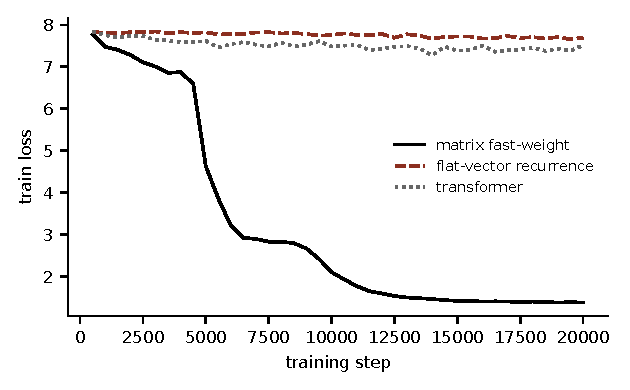
\includegraphics[width=0.62\linewidth]{figures/fig3_traincurve.pdf}
\caption{Training loss (primary task, seed 0) over the full
20{,}000-step run, all three arms, from the same archived configs used
for the parameter counts in Section~\ref{sec:setup}. The flat-vector and
transformer arms drop to 7.83 and 7.84 by step 500 and move only to 7.69
and 7.51 over the remaining 19{,}500 steps; the matrix fast-weight arm
keeps falling for the entire run, reaching
1.38. % <!-- evidence: C11 -->
Hyperparameters are the shared settings of Section~\ref{sec:setup}; no
per-architecture learning-rate sensitivity sweep was run, and
Section~\ref{sec:recall} scopes its claim to this shared budget
accordingly.}
\label{fig:traincurve}
\end{figure}

\section{Reproducibility of every number}
\label{app:repro}

Every figure and every table cell in this paper regenerates from archived
evaluation artifacts by a single versioned script that asserts the MD5
checksum of each source file before loading it; a changed artifact fails
the build rather than silently changing a number. Every inline numerical
claim in the source carries a machine-checkable comment naming its row in
a claims-to-evidence map maintained alongside the draft. The archived
artifacts, the script, and the map will be released with the
de-anonymized version of this paper.


\end{document}
